\documentclass[a4paper,11pt]{article}
\input{/home/tof/Documents/Cozy/latex-include/preambule_doc.tex}
\input{/home/tof/Documents/Cozy/latex-include/preambule_commun.tex}
\newcommand{\showprof}{show them}  % comment this line if you don't want to see todo environment
\setlength{\fboxrule}{0.8pt}
\fancyhead[L]{\fbox{\Large{\textbf{Secu 02}}}}
\fancyhead[C]{\textbf{Chiffrement asymétrique - Diffie-Hellman}}
\newdate{madate}{10}{09}{2020}
%\fancyhead[R]{\displaydate{madate}} %\today
%\fancyhead[R]{Seconde - SNT}
%\fancyhead[R]{Première - NSI}
\fancyhead[R]{Terminale - NSI}
\fancyfoot[L]{\vspace{1mm}Christophe Viroulaud}
\AtEndDocument{\label{lastpage}}
\fancyfoot[C]{\textbf{Page \thepage/\pageref{lastpage}}}
\fancyfoot[R]{\includegraphics[width=2cm,align=t]{/home/tof/Documents/Cozy/latex-include/cc.png}}
\usepackage{tikz}

\begin{document}
\section{Problématique}
Le chiffrement symétrique est très efficace mais il souffre d'un défaut majeur: il faut que la source et le destinataire utilise la même clé de chiffrement. La difficulté ici est donc de pouvoir s'échanger cette clé de manière sécurisée.
\begin{center}
    \framebox{Peut-on échanger une clé de manière sécurisée?}
\end{center}
\section{S'aider des mathématiques}
% 1974 puzzle merkle
\subsection{Principe}
Pour résoudre le problème de l'échange de clés \textbf{Diffie et Hellman}, deux cryptologues américains, proposent en 1976 une méthode pour convenir d'une clé symétrique partagée en passant par un canal non sécurisé. Cet algorithme s'appuie sur une fonction mathématique, notée \emph{f}, telle que:
\begin{itemize}
    \item La fonction $f$ est connue de tous.
    \item Si on connaît $f(x,y)$ et $x$ alors il est difficile de retrouver $y$.
    \item Pour tous entiers $x,y,z$, $f(f(x,y),z)=f(f(x,z),y)$
\end{itemize}
\subsection{Analogie des couleurs}
\begin{center}
    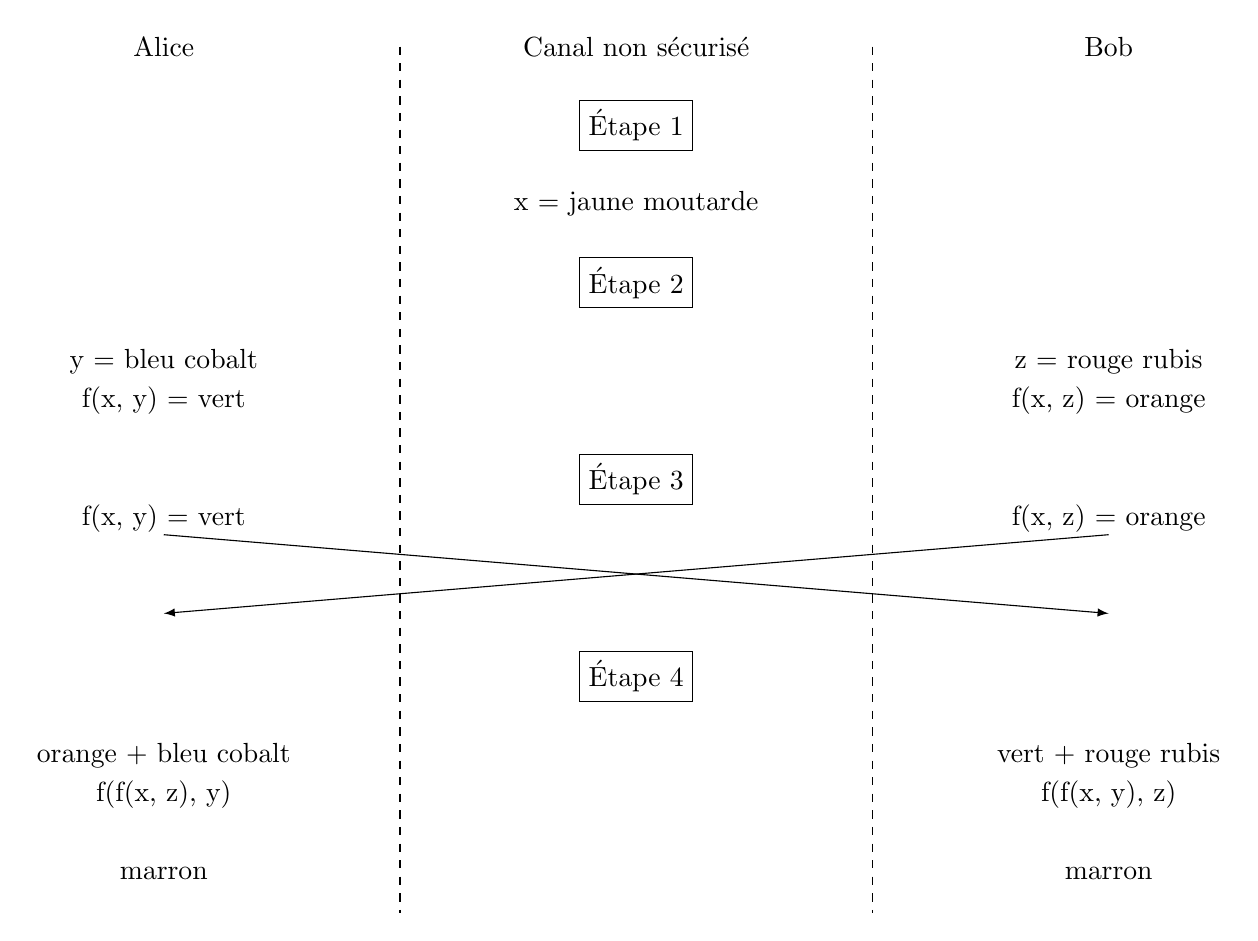
\begin{tikzpicture}
        \node at(-6,0){Alice};
        \node at(0,0){Canal non sécurisé};
        \node at(6,0){Bob};
        \draw[dashed] (-3,0) -- (-3,-11) ;
        \draw[dashed] (3,0) -- (3,-11) ;

        \node[draw] at(0,-1){Étape 1};
        \node at(0,-2){x = jaune moutarde};

        \node[draw] at(0,-3){Étape 2};
        \node at(-6,-4){y = bleu cobalt};
        \node at(6,-4){z = rouge rubis};
        \node at(-6,-4.5){f(x, y) = vert};
        \node at(6,-4.5){f(x, z) = orange};

        \node[draw] at(0,-5.5){Étape 3};
        \node at(-6,-6){f(x, y) = vert};
        \node at(6,-6){f(x, z) = orange};
        \draw[->,>=latex] (-6,-6.2) -- (6,-7.2);
        \draw[->,>=latex] (6,-6.2) -- (-6,-7.2);

        \node[draw] at(0,-8){Étape 4};
        \node at(-6,-9){orange + bleu cobalt};
        \node at(-6,-9.5){f(f(x, z), y)};
        \node at(6,-9){vert + rouge rubis};
        \node at(6,-9.5){f(f(x, y), z)};
        \node at(6,-10.5){marron};
        \node at(-6,-10.5){marron};

    \end{tikzpicture}
    \captionof{figure}{Analogie des couleurs}
\end{center}
% en pratique histoire de puissance et de modulo
\section{Faiblesse du protocole}
Il est mathématiquement très difficile pour Eve (\emph{eavesdropper: écouteuse}) de retrouver les valeurs choisies par Alice et Bob. Cependant, elle n'est pas obligée de le faire.
\begin{center}
    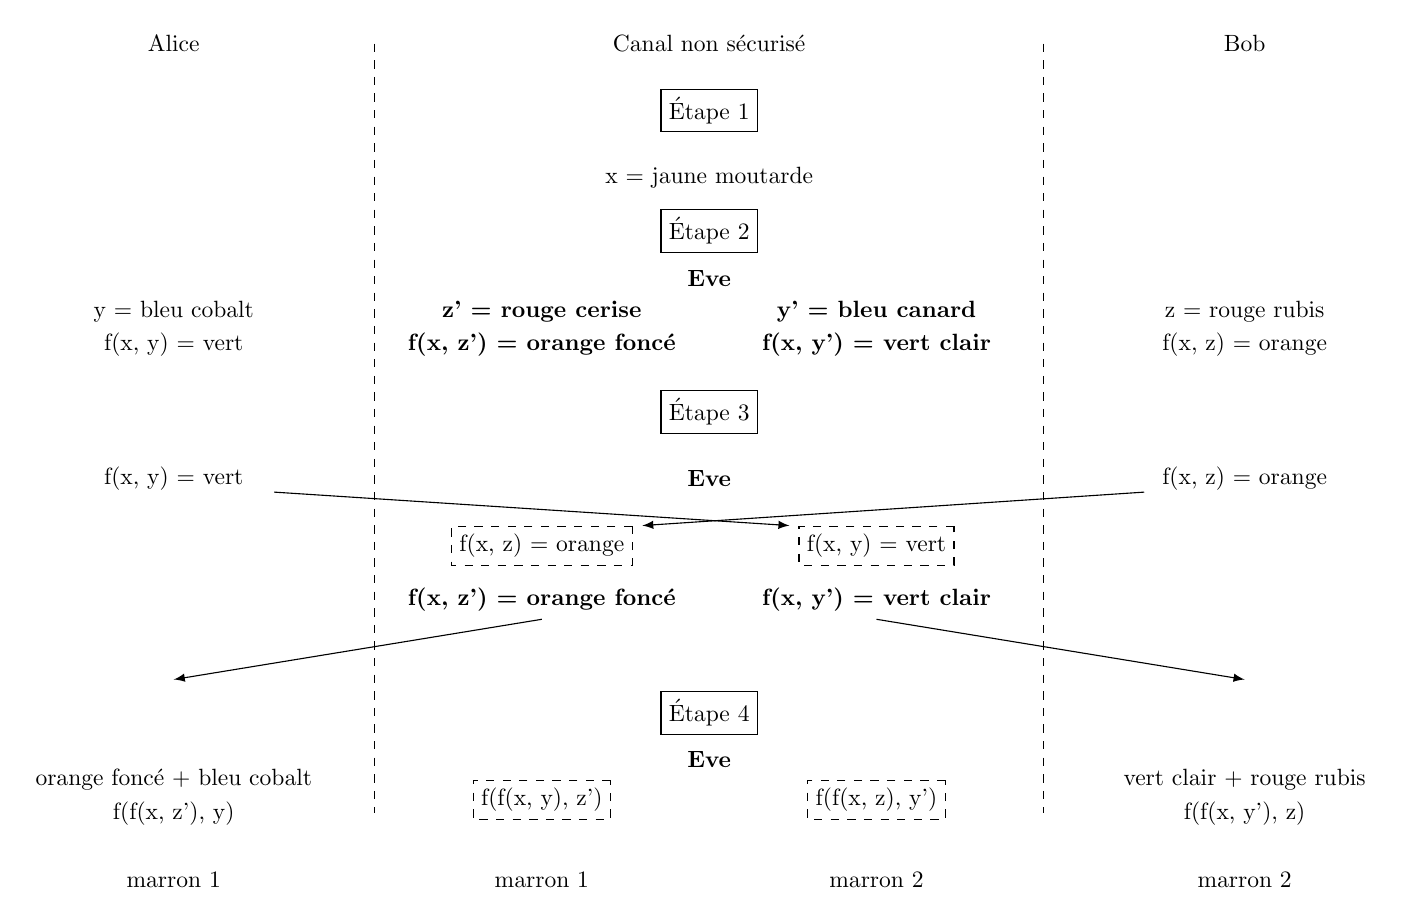
\begin{tikzpicture}[scale=0.85, transform shape]
        \node at(-8,0){Alice};
        \node at(0,0){Canal non sécurisé};
        \node at(8,0){Bob};
        \draw[dashed] (-5,0) -- (-5,-11.5) ;
        \draw[dashed] (5,0) -- (5,-11.5) ;

        \node[draw] at(0,-1){Étape 1};
        \node at(0,-2){x = jaune moutarde};

        \node[draw] at(0,-2.8){Étape 2};
        \node at(0,-3.5){\textbf{Eve}};
        \node at(2.5,-4){\textbf{y' = bleu canard}};
        \node at(2.5,-4.5){\textbf{f(x, y') = vert clair}};
        \node at(-2.5,-4){\textbf{z' = rouge cerise}};
        \node at(-2.5,-4.5){\textbf{f(x, z') = orange foncé}};
        \node at(-8,-4){y = bleu cobalt};
        \node at(8,-4){z = rouge rubis};
        \node at(-8,-4.5){f(x, y) = vert};
        \node at(8,-4.5){f(x, z) = orange};

        \node[draw] at(0,-5.5){Étape 3};
        \node at(0,-6.5){\textbf{Eve}};
        \node at(2.5,-8.3){\textbf{f(x, y') = vert clair}};
        \node at(-2.5,-8.3){\textbf{f(x, z') = orange foncé}};
        \node[draw, dashed] at(2.5,-7.5){f(x, y) = vert};
        \node[draw, dashed] at(-2.5,-7.5){f(x, z) = orange};
        \node at(-8,-6.5){f(x, y) = vert};
        \node at(8,-6.5){f(x, z) = orange};
        \draw[->,>=latex] (-6.5,-6.7) -- (1.2,-7.2);
        \draw[->,>=latex] (6.5,-6.7) -- (-1,-7.2);
        \draw[->,>=latex] (2.5,-8.6) -- (8,-9.5);
        \draw[->,>=latex] (-2.5,-8.6) -- (-8,-9.5);

        \node[draw] at(0,-10){Étape 4};
        \node at(0,-10.7){\textbf{Eve}};
        \node[draw, dashed] at(-2.5,-11.3){f(f(x, y), z')};
        \node[draw, dashed] at(2.5,-11.3){f(f(x, z), y')};
        \node at(-8,-11){orange foncé + bleu cobalt};
        \node at(-8,-11.5){f(f(x, z'), y)};
        \node at(8,-11){vert clair + rouge rubis};
        \node at(8,-11.5){f(f(x, y'), z)};
        \node at(-8,-12.5){marron 1};
        \node at(-2.5,-12.5){marron 1};
        \node at(2.5,-12.5){marron 2};
        \node at(8,-12.5){marron 2};

    \end{tikzpicture}
    \captionof{figure}{Attaque de l'homme du milieu}
\end{center}
\begin{aretenir}[]
Le protocole de Diffie-Hellman permet d'échanger des clés par un canal non sécurisé. Cependant il n'assure pas l'\emph{authentification} des participants.
\end{aretenir}
\end{document}